%!TEX root = draft.tex
\section{Checking Linearizability of Priority Queue Executions}
\label{sec:checking inclusion by recursive procedure}

%TODO REPHRASE THIS
%While checking linearizability of a given execution is known to be NP-complete in general~\cite{journals/siamcomp/GibbonsK97} we show in this section that it is polynomial-time for data-differentiated executions of the priority queue.
We define a recursive procedure for checking linearizability of an execution w.r.t. $\seqPQ$.
To ease the exposition, Section~\ref{ssec:seq_exec} introduces a recursive procedure for checking whether a data-differentiated \emph{sequential} execution is admitted by the priority queue which is then extended to the concurrent case in Section~\ref{ssec:conc_exec}.

\subsection{Characterizing Data-Differentiated Sequential Executions}\label{ssec:seq_exec}

Checking whether a data-differentiated sequential execution belongs to $\seqPQ$ could be implemented by checking membership into the language accepted by the LTS $PQ$. The recursive procedure $\textit{Check-PQ-Seq}$ outlined in Algorithm~\ref{alg:seq_check} is an alternative to this membership test. Roughly, it selects one or two operations in the input execution, checks whether their return values are correct by ignoring the order between the other operations other than how they are ordered w.r.t. the selected ones, and calls itself recursively on the execution without the selected operations. %{\color {blue} Here we implicitly mix operation $o$ (when $\textit{call}_o(m,a)$, $\textit{ret}_o(m,b)$ in $e$) with $m(a,b)$.}

We explain how the procedure works on the following execution:
\begin{align}
\hspace{-5mm}\textit{put}(c,p_2) \cdot \textit{put}(a,p_1) \cdot \textit{rm}(a) \cdot \textit{rm}(c) \cdot \textit{rm}(\textit{empty}) \cdot \textit{put}(d,p_2) \cdot \textit{put}(e,p_3) \cdot \textit{rm}(e) \cdot \textit{put}(b,p_1)\label{eq:ex_rec1}
\end{align}
where $p_1$, $p_2$, $p_3$ are priorities such that $p_1 \prec p_2$ and $p_1 \prec p_3$, and $p_2$ and $p_3$ are incomparable. Since the $\textit{rm}(\textit{empty})$ operations\footnote{An $m(a)$-operation in an execution $e$ is an operation identifier $o$ s.t. $e$ contains the actions $\textit{call}_o(m,a)$, $\textit{ret}_o(m,a)$.} are read-only (they don't affect the state of the queue), they are selected first. Ensuring that an operation $o=\textit{rm}(\textit{empty})$ is correct boils down to checking that every $\textit{put}(x,p)$ operation before $o$ is matched to a $\textit{rm}(x)$ operation which also occurs before $o$. This is true in this case for $x\in \{a,c\}$. Therefore, the correctness of (\ref{eq:ex_rec1}) reduces to the correctness of
\begin{align*}
\textit{put}(c,p_2) \cdot \textit{put}(a,p_1) \cdot \textit{rm}(a) \cdot \textit{rm}(c) \cdot \textit{put}(d,p_2) \cdot \textit{put}(e,p_3) \cdot \textit{rm}(e) \cdot \textit{put}(b,p_1)
\end{align*}
When there are no more $\textit{rm}(\textit{empty})$ operations, the procedure selects a $\textit{put}$ operation adding a value with maximal priority which is not removed, and then a pair of $\textit{put}$ and $\textit{rm}$ operations adding and removing the same maximal priority value. For instance, since $p_2$ is a maximal priority, it may select the operation $\textit{put}(d,p_2)$. {This operation is correct if $d$ is the last value with priority $p_2$, and the correctness of (\ref{eq:ex_rec1}) reduces to the correctness of
\begin{align*}
\textit{put}(c,p_2) \cdot \textit{put}(a,p_1) \cdot \textit{rm}(a) \cdot \textit{rm}(c) \cdot \textit{put}(e,p_3) \cdot \textit{rm}(e) \cdot \textit{put}(b,p_1)
\end{align*}
Since there is no other value of priority $p_2$ which is not removed, the procedure selects a pair of $\textit{put}$/$\textit{rm}$ operations with an argument of priority $p_2$,} for instance, $\textit{put}(c,p_2)$ and $\textit{rm}(c)$. The value returned by $\textit{rm}$ is correct if all the values of priority smaller than $p_2$ added before $\textit{rm}(c)$ are also removed before $\textit{rm}(c)$. In this case, $a$ is the only value of priority smaller than $p_2$ and it satisfies this property. Applying a similar reasoning for all the remaining values, it can be proved that this execution is correct.

\begin{algorithm}[t]
\KwIn {A data-differentiated sequential execution $e$}
\KwOut{$\mathsf{true}$ iff $e\in \seqPQ$}

\If {$e = \epsilon$}
{\Return $\mathsf{true}$\;}

\If {$\mathsf{Has\text{-}EmptyRemoves}(e)$}
{
    \If {$\exists\ o=\textit{rm}(\textit{empty})\in e$ such that $\mathsf{EmptyRemove\text{-}Seq}(e,o)$ holds}
    {
        \KwRet $\textit{Check-PQ-Seq}(e \setminus o)$\;
    }
    %\Else {\KwRet $\mathsf{false}$\;}
}
\ElseIf{$\mathsf{Has\text{-}UnmatchedMaxPriority}(e)$}
{
    \If {$\exists\ x \in \textit{values}(e)$ such that $\mathsf{UnmatchedMaxPriority\text{-}Seq}(e,x)$ holds}
    {
        \KwRet $\textit{Check-PQ-Seq}(e \setminus x)$\;
    }
    %\Else {\KwRet $\mathsf{false}$\;}
}

\Else
{
    \If {$\exists\ x \in \textit{values}(e)$ such that $\mathsf{MatchedMaxPriority\text{-}Seq}(e,x)$ holds}
    {
        \KwRet $\textit{Check-PQ-Seq}(e \setminus x)$\;
    }
    \Else {\KwRet $\mathsf{false}$\;}
}
\caption{$\textit{Check-PQ-Seq}$}
\label{alg:seq_check}
\end{algorithm}


In formal terms, the operations which are selected depend on the following set of predicates on executions:
{\small
\begin{align*}
\mathsf{Has\text{-}EmptyRemoves}(e)=\mathsf{true} & \mbox{ iff  $e$ contains a $\textit{rm}(\textit{empty})$ operation} \\
\mathsf{Has\text{-}UnmatchedMaxPriority}(e)=\mathsf{true} & \mbox{ iff $p\in \textit{unmatched-priorities}(e)$ for a maximal priority} \\
&\hspace{4mm}\mbox{$p\in priorities(e)$}
\end{align*}}
where $\textit{priorities}(l)$, resp., $\textit{unmatched-priorities}(l)$, is the set of priorities occurring in $\textit{put}$ operations of $e$, resp., in $\textit{put}$ operations of $e$ for which there is no $\textit{rm}$ operation removing the same value. We call the latter \emph{unmatched} put operations. A put operation which is not unmatched is called \emph{matched}. For simplicity, we consider the following syntactic sugar $\mathsf{Has\text{-}MatchedMaxPriority}(e)=\neg \mathsf{Has\text{-}EmptyRemoves}(e)\land \neg \mathsf{Has\text{-}UnmatchedMaxPriority}(e)$. By an abuse of notation, we also assume that  $\mathsf{Has\text{-}UnmatchedMaxPriority}(e) \Rightarrow \neg \mathsf{Has\text{-}EmptyRemoves}(e)$ (this is sound by the order of the conditionals in $\textit{Check-PQ-Seq}$.

The predicates defining the correctness of the selected operations are defined as follows:
{\small
\begin{align*}
\mathsf{EmptyRemove\text{-}Seq}(e,o)=\mathsf{true} & \mbox{ iff  $e= u\cdot o\cdot v$ and $\textit{matched}(u)$} \\
\mathsf{UnmatchedMaxPriority\text{-}Seq}(e,x)=\mathsf{true} & \mbox{ iff  $e= u\cdot \textit{put}(x,p)\cdot v$, $p\not\prec \textit{priorities}(u\cdot v)$, and $p\not\in \textit{priorities}(v)$} \\
\mathsf{MatchedMaxPriority\text{-}Seq}(e,x)=\mathsf{true} & \mbox{ iff  $e= u\cdot \textit{put}(x,p)\cdot v\cdot \textit{rm}(x)\cdot w$, $p\not\prec \textit{priorities}(u\cdot v\cdot w)$,} \\
&\hspace{4mm}\mbox{$p\not\preceq \textit{unmatched-priorities}(u\cdot v\cdot w)$, $\textit{matched}_\prec(u\cdot v,p)$,} \\
&\hspace{4mm}\mbox{and $p\not\in \textit{priorities}(v\cdot w)$}
\end{align*}
}

\vspace{-3mm}
\noindent
where $p\prec \textit{priorities}(e)$ when $p\prec p'$ for some $p'\in \textit{priorities}(e)$ (and similarly for $p\prec \textit{unmatched-priorities}(e)$ or $p\preceq \textit{unmatched-priorities}(e)$),
$\textit{matched}_\prec(e,p)$ holds when each value with priority strictly smaller than $p$ is removed in $e$, and $\textit{matched}(e)$ holds when $\textit{matched}_\prec(e,p)$ holds for each $p\in\mathbb{P}$. Compared to the example presented at the beginning of the section, these predicates take into consideration that multiple values with the same priority are removed in FIFO order: the predicate $\mathsf{MatchedMaxPrioritySeq}(e,x)$ holds when $x$ is the last value with priority $p$ added in $e$.

When $o$ is a $\textit{rm}(\textit{empty})$ operation, we write $e\setminus o$ for the maximal subsequence of $e$ which doesn't contain $o$. For an execution $e$, $\textit{values}(e)$ is the set of values occurring in call/return actions of $e$.


% and items of unmatched put in $l$, respectively. $p \prec \textit{priorities}(l)$ (resp., $p \preceq \textit{priorities}(l)$), if $p \prec p'$ (resp., $p \preceq p'$)for some $p' \in \textit{priorities}(l)$. Similarly we can define $p \preceq \textit{unmatched-priorities}(l)$.
%
%
%Essentially, this procedure chooses either a $\textit{rm}(\textit{empty})$ operation or a set of operations adding/removing a maximal priority in the input execution and checks whether they satisfy certain properties
%
%
% proceeds by
%
% The projection $e \vert{O}$ of $e$ into $O$ is obtained from $e$ by erasing all call and return actions of non-$O$ operations. We write $e \setminus o$ for the projection $e \vert_{ O_e \setminus \{ o \} }$, where $O_e$ is the set of operations of $e$.
%
%Given a data-differentiated sequential execution $e$, it is costly to check whether $e$ belongs to priority queue, since for each element of $e$, we should keep the current content of priority queue and try to modify the priority queue according to this element. Such process is too complex. In this section, we propose another method for checking inclusion of priority queue by using a recursive procedure $\textit{check-PQ}$. For checking a sequence, every time we only check a much simpler property, and then recursively check the remanning sequences obtained by erasing one or two elements. Each step of our method is easier to deal with.
%
%$\textit{put}(a,p)$ matches $\textit{rm}(b)$, if $a = b$. To introduce $\textit{check-PQ}$, let us introduce several predicates. Given sequential execution $l$ and priority $p$:
%
%\begin{itemize}
%\setlength{\itemsep}{0.5pt}
%\item[-] $\textit{rm}(\textit{empty}) \notin l$ is satisfied when $l$ does not contain $\textit{rm}(\textit{empty})$.
%
%\item[-] Let $\textit{priorities}(l)$ and $\textit{unmatched-priorities}(l)$ be the set of priorities of putted items and items of unmatched put in $l$, respectively. $p \prec \textit{priorities}(l)$ (resp., $p \preceq \textit{priorities}(l)$), if $p \prec p'$ (resp., $p \preceq p'$)for some $p' \in \textit{priorities}(l)$. Similarly we can define $p \preceq \textit{unmatched-priorities}(l)$.
%
%\item[-] $\textit{matched}_{\prec}(l,p)$ is satisfied, if for each item of $l$ with priorities smaller than $p$, it has matched $\textit{put}$ and $\textit{rm}$. Similarly, we can define $\textit{matched}(l)$, where we consider all items in $l$ instead of items with certain priorities.
%\end{itemize}
%
%Let us introduce some notations: given sequential executions $u,v,w$ and priority $p$,
%
%\begin{itemize}
%\setlength{\itemsep}{0.5pt}
%\item[-] $\textit{PQ}_1(u,v,w,p) \equiv
%(\textit{rm}(\textit{empty}) \notin u \cdot v \cdot w) \wedge
%(p \not\prec \textit{priorities}(u \cdot v \cdot w)) \wedge
%(p \not\preceq \textit{unmatched-priorities}(u \cdot v \cdot w)) \wedge
%(\textit{matched}_{\prec}(u \cdot v,p) ) \wedge
%(p \notin \textit{priorities}(v \cdot w))$
%
%\item[-] $\textit{PQ}_2(u,v,p) \equiv
%(\textit{rm}(\textit{empty}) \notin u \cdot v) \wedge
%(p \not\prec \textit{priorities}(u \cdot v \cdot w)) \wedge
%(p \notin \textit{priorities}(v \cdot w))$
%
%\item[-] $\textit{PQ}_3(u,v) \equiv
%\textit{matched}(u \cdot v)$
%\end{itemize}
%
%
%Let us defined set $\textit{MS}(R)$ ($R \in \textit{PQ}_1,\textit{PQ}_2,\textit{PQ}_3$), which is the set of data-differentiated sequential executions that respect $R$.
%
%\begin{itemize}
%\setlength{\itemsep}{0.5pt}
%\item[-] $e \in \textit{MS}(\textit{PQ}_1)$, if $e = u \cdot \textit{put}(x,p) \cdot v \cdot \textit{rm}(x) \cdot w$ and $\textit{PQ}_1(u,v,w,p)$ holds for some item $x$ and a maximal priority $p$,
%
%\item[-] $e \in \textit{MS}(\textit{PQ}_2)$, if $e = u \cdot \textit{put}(x,p) \cdot v$ and $\textit{PQ}_2(u,v,p)$ holds for some item $x$ and a maximal priority $p$,
%
%\item[-] $e \in \textit{MS}(\textit{PQ}_3)$, if $e = u \cdot \textit{rm}(\textit{empty}) \cdot v$ and $\textit{PQ}_3(u,v)$ holds.
%\end{itemize}
%
%We call such $x$ and $\textit{rm}(\textit{empty})$ (if exists) the witness of $e$. Note that sequences in $\textit{MS}(R)$ does not guaranteed to be a priority queue execution. Let us introduce the notion $\textit{last}(e)$, which is a set and used as the branch condition of $\textit{check-PQ}$. Here $e$ is a data-differentiated sequential execution.
%
%\begin{itemize}
%\setlength{\itemsep}{0.5pt}
%\item[-] If $e$ contains $\textit{rm}(\textit{empty})$, then $\textit{last}(e) = \{ \textit{PQ}_3 \}$.
%
%\item[-] Else, if for a maximal priority $p$ of $e$, $\textit{unmatched-priorities}(e) \neq \emptyset$, then $\textit{PQ}_2 \in \textit{last}(e)$.
%
%\item[-] Else, if for a maximal priority $p$ of $e$, $\textit{unmatched-priorities}(e) = \emptyset$, then $\textit{PQ}_1 \in \textit{last}(e)$.
%\end{itemize}
%
%When $\textit{last}(e)$ contains only one element $R$, we write $\textit{last}(w)=R$ for simplicity.
%
%The projection $e \vert{\mathcal{D}}$ of $e$ into $\mathcal{D} \subseteq \mathbb{D}$ is obtained from $e$ by erasing all elements with a data value not in $\mathcal{D}$. We write $e \setminus x$ for the projection $e \vert_{ \mathbb{D} \setminus \{ x \} }$. The projection $e \vert{O}$ of $e$ into $O$ is obtained from $e$ by erasing all call and return actions of non-$O$ operations. We write $e \setminus o$ for the projection $e \vert_{ O_e \setminus \{ o \} }$, where $O_e$ is the set of operations of $e$.
%
%The recursive procedure $\textit{con-check-EPQ}$ is given as follows. Here $P_i(e,o)$ and $P_i(e,x)$ is the predicates of $e \in \textit{MS}(\textit{PQ}_i)$ withe witness $o$ or $x$, respectively.
%
%\begin{minipage}{.5\textwidth}
%\begin{algorithm}[H]
%\KwIn {a data-differentiated sequential execution $e$}
%
%\If {$e = \epsilon$}
%{\KwRet $\textit{true}$;}
%
%\If {$\textit{last}(e) = \textit{PQ}_3$}
%{
%    \If {$\exists o=\textit{rm}(\textit{empty})$, $P_3(e,o)$ holds}
%    {
%        \KwRet $\textit{check-PQ}(e \setminus o)$;
%    }
%    \KwRet $\textit{false}$;
%}
%
%\If {$\textit{PQ}_i \in \textit{last}(e)$ for $i \in \{1,2\}$}
%{
%    \If {$\exists l$, $P_i(e,x)$ holds}
%    {
%        \KwRet $\textit{check-PQ}(e \setminus x)$;
%    }
%    \KwRet $\textit{false}$;
%}
%\caption{$\textit{check-PQ}$}
%\label{Method-check-PQ}
%\end{algorithm}
%\end{minipage}
%\hfill


%TODO MODIFY THE FOLLOWING EXAMPLE
%
%Let us use an example to show how $\textit{check-PQ}$ works. Here we use $w_1 \xrightarrow{R} w_2$ to denote that in $\textit{check-PQ}(w_1)$, we choose the branch of $R$ and recursively call $\textit{check-PQ}(w_2)$.
%
%\begin{example}\label{example:generate extended priority queue executions}
%Given priorities $p_1,p_2,p_3$ with orders $p_1 \prec p_2$ and $p_1 \prec p_3$,
%
%\noindent $\textit{put}(c,p_2) \cdot \textit{put}(a,p_1) \cdot \textit{rm}(a) \cdot \textit{rm}(c) \cdot \textit{rm}(\textit{empty}) \cdot \textit{put}(d,p_2) \cdot \textit{put}(e,p_3) \cdot \textit{rm}(e) \cdot \textit{put}(b,p_1)$
%
%$\xrightarrow{\textit{EPQ}_3}$ $\textit{put}(c,p_2) \cdot \textit{put}(a,p_1) \cdot \textit{rm}(a) \cdot \textit{rm}(c) \cdot \textit{put}(d,p_2) \cdot \textit{put}(e,p_3) \cdot \textit{rm}(e) \cdot \textit{put}(b,p_1)$
%
%$\xrightarrow{\textit{EPQ}_1}$ $\textit{put}(c,p_2) \cdot \textit{put}(a,p_1) \cdot \textit{rm}(a) \cdot \textit{rm}(c) \cdot \textit{put}(d,p_2) \cdot \textit{put}(b,p_1)$
%
%$\xrightarrow{\textit{EPQ}_2}$ $\textit{put}(c,p_2) \cdot \textit{put}(a,p_1) \cdot \textit{rm}(a) \cdot \textit{rm}(c) \cdot \textit{put}(b,p_1)$
%
%$\xrightarrow{\textit{EPQ}_1}$ $\textit{put}(a,p_1) \cdot \textit{rm}(a) \cdot \textit{put}(b,p_1)$
%
%$\xrightarrow{\textit{EPQ}_2}$ $\textit{put}(a,p_1) \cdot \textit{rm}(a)$
%
%$\xrightarrow{\textit{EPQ}_1}$ $\epsilon$
%\end{example}

The following lemma states the correctness of $\textit{Check-PQ-Seq}$ (the proof can be found in Appendix~\ref{sec:appendix definition of seqPQ and proof of Lemma EQP rules and semantics}).

\begin{restatable}{lemma}{EPQRulesAndSemantics}
\label{lemma:EPQ rules and semantics}
$\textit{Check-PQ-Seq}(e)=\mathsf{true}$ iff $e\in \seqPQ$, for every data-differentiated sequential execution $e$.
\end{restatable}

%
%\begin{lemma}
%Algorithm~\ref{alg:seq_check} returns $\mathsf{true}$ on an execution $e$ iff $e\in \seqPQ$.
%\end{lemma}


%Let $\textit{PQ}$ be set of sequences obtained by renaming some data-differentiated sequential execution that is accepted by $\textit{check-PQ}$. To persuade readers that $\textit{PQ}$ is indeed the set of behaviors of priority queue, in Appendix \ref{sec:appendix in section inductive rules of extended priority queue}, we give a semantical version definition $\textit{PQ}_s$ of priority queue, and shows that $\textit{PQ} = \textit{PQ}_s$. To model the possible behaviors of priority queue, we model it as an labelled transition system (shortened as LTS) $\textit{LTS}_e$. Each state of $\textit{LTS}_e$ is a function from $\mathbb{P}$ into sequences over $\mathbb{D}$, and represents a snapshot of contents of priority queue. $\textit{PQ}_s$ is the set of traces of $\textit{LTS}_e$. The definition of $\textit{PQ}_s$ and the proof of the following lemma can be found in Appendix \ref{sec:appendix in section inductive rules of extended priority queue}.
%
%\begin{restatable}{lemma}{EPQRulesAndSemantics}
%\label{lemma:EPQ rules and semantics}
%$\textit{PQ} = \textit{PQ}_s$.
%\end{restatable}
%
%By Example \ref{example:generate extended priority queue executions} we can see how to generate a sequence $e \in \textit{EP}$ from $\epsilon$ as follows:
%
%\begin{itemize}
%\setlength{\itemsep}{0.5pt}
%\item[-] First we add non-$\textit{rm}(\textit{empty})$ elements with a loop: Let $P$ be the set of priorities of items in $e$. In the first round of the loop, we choose a minimal priorities $p \in P$, we add items by using $\textit{PQ}_1$ and $\textit{PQ}_2$, let $P = P \setminus \{p\}$, and begins the next round of loop.
%
%\item[-] Then, we add $\textit{rm}(\textit{empty})$ by using $\textit{PQ}_3$.
%\end{itemize}

\subsection{Checking Linearizability of Data-Differentiated Concurrent Executions}\label{ssec:conc_exec}

The extension of $\textit{Check-PQ-Seq}$ to concurrent executions, checking whether they are linearizable w.r.t. $\seqPQ$, is obtained by replacing every predicate $\Gamma\mathsf{\text{-}Seq}$ with
\begin{align*}
\Gamma\mathsf{\text{-}Conc}(e,\alpha) = \mathsf{true}\mbox{ iff there exists a sequential execution $s$ such that $e\sqsubseteq s$ and $\Gamma\mathsf{\text{-}Seq}(s,\alpha)$}
\end{align*}
for each $\Gamma\in \{\mathsf{EmptyRemove}, \mathsf{UnmatchedMaxPriority}, \mathsf{MatchedMaxPriority}\}$. Let $\textit{Check-PQ-Conc}$ denote the thus obtained procedure (we assume recursive calls are modified accordingly).

% with linearizability to deal with linearizability w.r.t $\textit{PQ}$ as follows:
%
%\begin{itemize}
%\setlength{\itemsep}{0.5pt}
%\item[-] The input $e$ is a concurrent execution.
%
%\item[-] $\textit{last}(e)$ is the union of $\textit{last}(u)$ for any sequential execution $u$ such that $e \sqsubseteq u$. $e \sqsubseteq \textit{MS}(R)$ with witness $x$ (resp., $o$), if $e \sqsubseteq u \in \textit{MS}(R)$ and $x$ (resp., $o$) is the witness of $u$.
%
%\item[-] $P_i(e,o)$ and $P_i(e,x)$ holds, if $e \sqsubseteq \textit{MS}(\textit{PQ}_i)$ withe witness $o$ or $x$, respectively.
%\end{itemize}

The following lemma states the correctness of $\textit{Check-PQ-Conc}$. Completeness follows easily from the properties of $\seqPQ$. Thus, if $\textit{Check-PQ-Conc}(e) = \textit{false}$, then there exists a set $D$ of values s.t. either  $\mathsf{EmptyRemove\text{-}Conc}(e \vert D)$ is false, or $\mathsf{UnmatchedMaxPriority\text{-}Conc}(e \vert D,x)$ is false for all the values $x$ of maximal priority that are not removed (and there exists at least one such value), or $\mathsf{MatchedMaxPriority\text{-}Conc}(e \vert D,x)$ is false for all the values $x$ of maximal priority (and these values are all removed in $e \vert D$). It can be easily seen that we get $e \vert D\not\sqsubseteq \seqPQ$ in all cases, which by the closure under projection of $\seqPQ$ implies, $e \not\sqsubseteq \seqPQ$ (since every linearization of $e$ includes as a subsequence a linearization of $e \vert D$).

\begin{restatable}{lemma}{ConCheckEPQIsCorrect}
\label{lemma:con-check-EPQ is correct}
$\textit{Check-PQ-Conc}(e)=\mathsf{true}$ iff $e \sqsubseteq \seqPQ$, for every data-differentiated execution $e$.
\end{restatable}


Proving soundness is highly non-trivial and one of the main technical contributions of this paper (see Appendix~\ref{sec:appendix subsection proof of lemma con-check-EPQ is correct} for a complete proof). The main technical difficulty is showing that for any execution $e$, any linearization of $e\setminus x$ for some maximal priority value $x$ can be extended to a linearization of $e$ provided that $\mathsf{UnmatchedMaxPriority}$ or $\mathsf{MatchedMaxPriority}$ holds (depending on whether there are values with the same priority as $x$ in $e$ which are not removed).
%
%
%To ensure that $\textit{check-PQ}(e) = \textit{true} \Rightarrow e \sqsubseteq \textit{PQ}$, we require $\textit{PQ}$ to satisfy the following property.
%
%for any data-differentiated execution $e$,
%\begin{itemize}
%\setlength{\itemsep}{0.5pt}
%\item[-] if $e \sqsubseteq \textit{MS}(R)$ ($R \in \{ \textit{PQ}_1, \textit{PQ}_2 \}$) with witness $x$, we have: $e \setminus x \sqsubseteq \textit{PQ} \Rightarrow e \sqsubseteq \textit{PQ}$.
%
%\item[-] if $e \sqsubseteq \textit{MS}(\textit{PQ}_3)$ and $o$ is a $\textit{rm}(\textit{empty})$, we have: $e \setminus o \sqsubseteq \textit{PQ} \Rightarrow e \sqsubseteq \textit{PQ}$.
%\end{itemize}
%
%With this property, we can build a linearization of a whole execution by increasingly construct linearization of sub-execution from $\epsilon$, and this convince us that $\textit{check-PQ}(e) = \textit{true} \Rightarrow e \sqsubseteq \textit{PQ}$.
%

Let us briefly explain the idea of proving this property when $\mathsf{MatchedMaxPriority}$ holds with an example. Assume $e \sqsubseteq l=u \cdot \textit{put}(x,p) \cdot v \cdot \textit{rm}(x) \cdot w$, $\mathsf{MatchedMaxPriority}(l,x)$ holds, and $e \setminus x \sqsubseteq l' \in \textit{PQ}$, as shown in \figurename~\ref{fig:concurrent execution for EPQ1} (a), we explicitly construct a sequence $l''= l''_1 \cdot \textit{put}(x,p) \cdot l''_2 \cdot \textit{rm}(x) \cdot l''_3$ and prove that $e \sqsubseteq l'' \in \textit{PQ}$. In this example, $p_1 \prec p$, $p_1 \prec p_2$, $u=\epsilon$, $w$ contains $\textit{rm}(z_2), \textit{put}(x_3,p_2), \textit{rm}(z_1)$ (emphasize by $\textit{rm}(z_2)-w$), and the remanning operations are in $v$. We also explicitly draw the linearization points according to $l'$. We construct $l''$ as follows, and this method does not rely on the locations of linearization points of $l'$ and operations of $x$.

\begin{itemize}
\setlength{\itemsep}{0.5pt}
\item[-] Let $p$-comparable operations (resp., $p$-incomparable operations) be the set of operations with items whose priority is comparable with $p$ (resp., incomparable with $p$). It seems that we can construct $l''_1$, $l''_2$ and $l''_3$ as the projection of $l'$ into operations of $u$, $v$ and $w$, respectively. However, this is incorrect, since $\mathsf{MatchedMaxPriority}(l,x)$ has no restriction to $p$-incomparable operations operations in $u \cdot v$, and thus, there is no guarantee that the projection of $l'$ into $p$-incomparable operations operations in $u \cdot v$ being correct. In this example, such projection is $\textit{put}(z_1,p_3) \cdot \textit{rm}(z_2)$ and is incorrect.

\item[-] Let us construct sets $U'$, $V'$ and $W'$, such then make $l''_1$, $l''_2$ and $l''_3$ the projections of $l'$ into $U'$, $V'$ and $W'$, respectively. This contains two steps:

\item[-] The first step is to define $W'$. The $p$-comparable operations in $W'$ is same as that in $w$. To obtain $p$-incomparable operations in $W'$, we try to find a $p$-incomparable operation $o$ which either happens before some $p$-comparable operations in $w$, or with linearization points after $\textit{rm}(x)$. Then, we put $o$ and all $p$-incomparable operations after $o$ in $l'$ into $W'$ (emphasized by boxes in example). In this example, $o$ is $\textit{rm}(z_1)$, and $p$-incomparable operations after $o$ in $l'$ is $\textit{rm}(z_2)$, which are emphasized by adding boxes. In this process, whether a $p$-incomparable operation is in $W'$ or not only relies whether it is before or after $o$ in $l'$.

\item[-] The second step is to define $U'$ and $V'$. $U'$ contains the following two kinds of operations: (1) Operations whose linearization points are before $\textit{ret}(\textit{put},x)$, and (2) other $\textit{put}$ operations with priority $p$. $V'$ contains the remanning operations. In this example, $U'$ contains $\textit{put}(z_1,p_3)$ and $\textit{put}(x_2,p_2)$.

\item[-] In this example, $l''_1 = \textit{put}(z_1,p_2) \cdot \textit{put}(x_2,p)$, $l''_2 = \textit{put}(z_2,p_2) \cdot \textit{rm}(x_2) \cdot \textit{put}(y_1,p_1) \cdot \textit{rm}(y_1)$, and $l''_3 = \textit{put}(x_3,p) \cdot \textit{rm}(z_1) \cdot \textit{rm}(z_2)$. In \figurename~\ref{fig:concurrent execution for EPQ1} (b), we add linarization points according to $l''$, and we can see that $l''$ holds as required.
\end{itemize}


%\begin {proof} (Sketch)
%It is not hard to see that $\textit{check-PQ}(e) = \textit{false} \Rightarrow e \not\sqsubseteq \textit{PQ}$, since $\textit{PQ}_{\neq} \subset \textit{MS}(R)_{\neq}$.


%This completes the proof of this lemma.
%
%
%\qed
%\end {proof}



\begin{figure}[t]
  \centering
  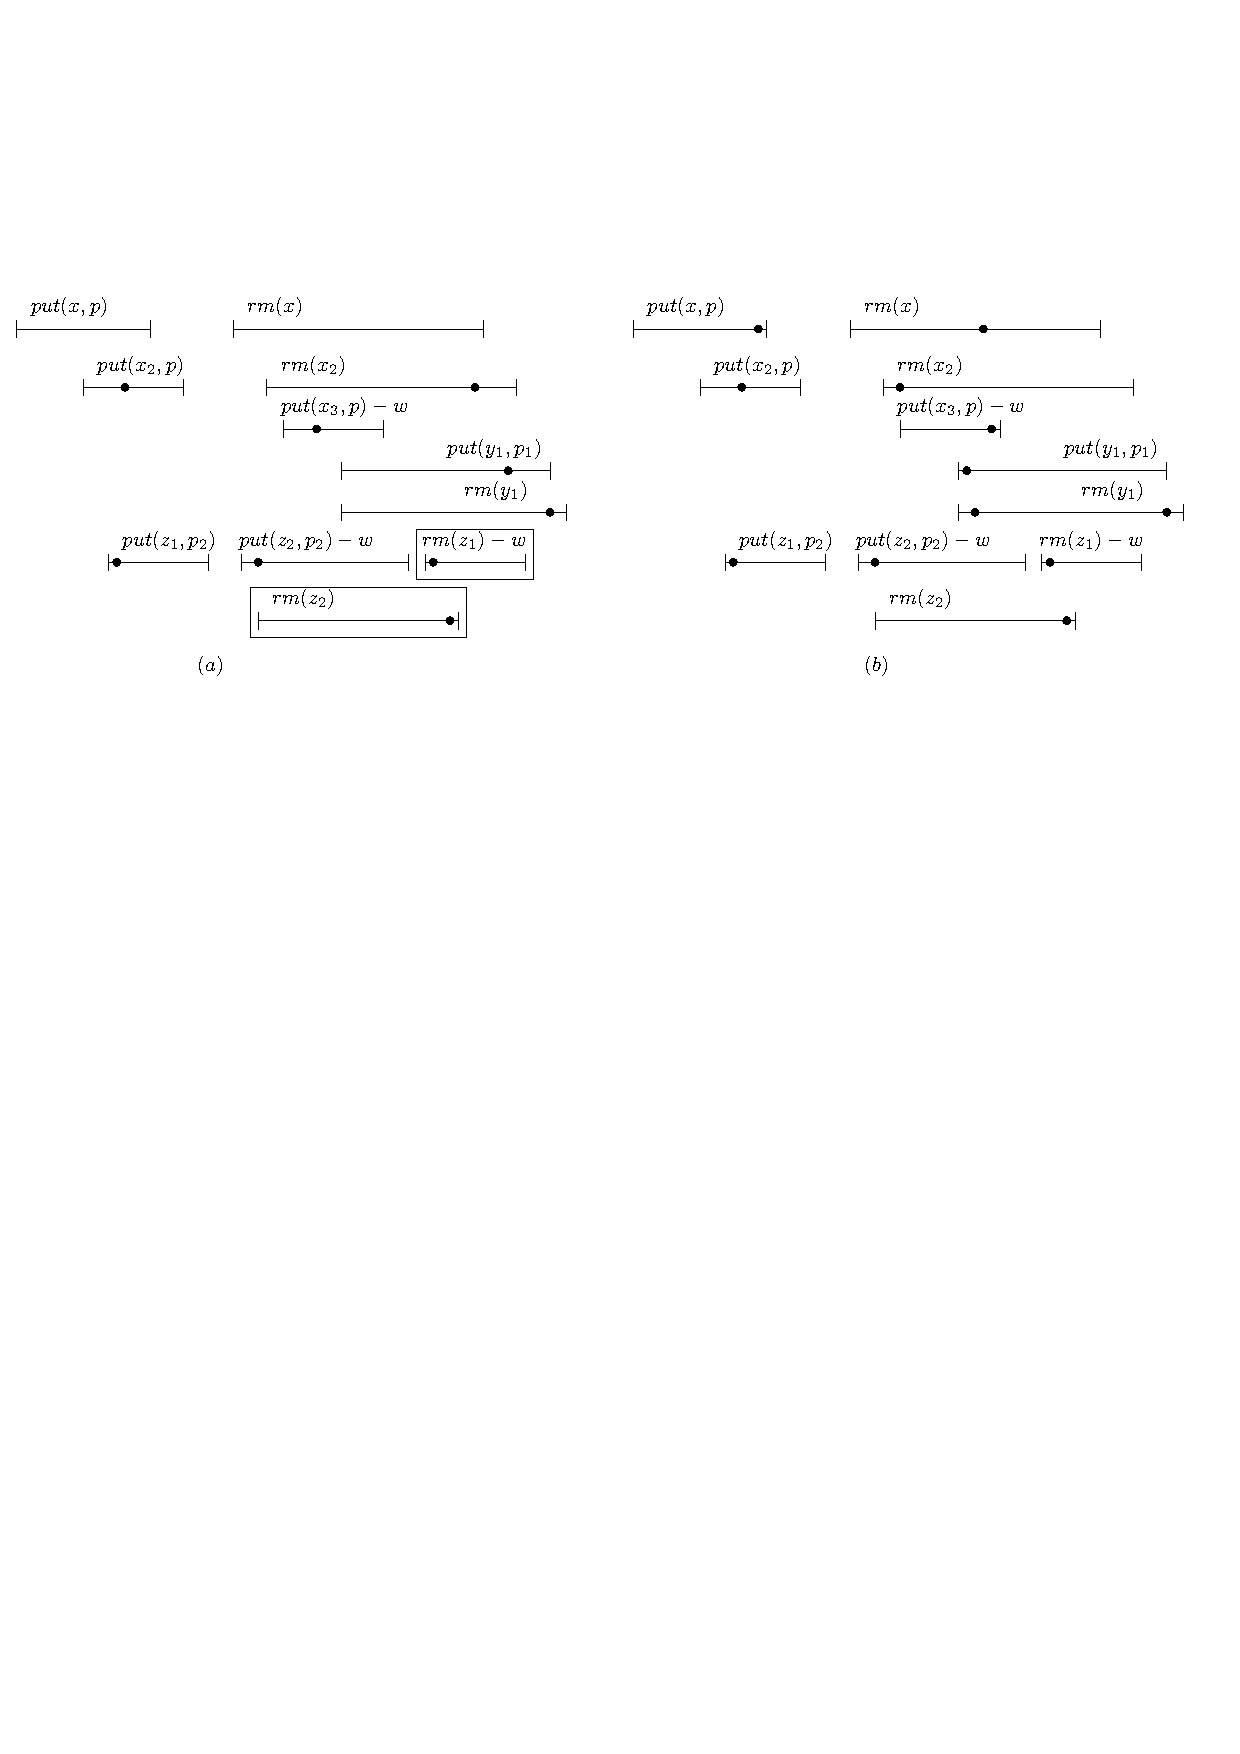
\includegraphics[width=1 \textwidth]{figures/PIC-HIS-EPQ1-TwoHis.pdf}
%\vspace{-10pt}
  \caption{The process of obtaining linearization of $e$}
  \label{fig:concurrent execution for EPQ1}
\end{figure}

Section~\ref{sec:co-regular of extended priority queues} introduces a characterization of concurrent priority queue violations using a set of \emph{non-recursive} automata (i.e., whose states consist of a fixed number of registers) whose product is equivalent to $\textit{Check-PQ-Conc}$ (modulo renaming of values which is possible by data-independence). Since $\seqPQ$ is closed under projection (Lemma~\ref{lem:closure_proj}), the recursion in $\textit{Check-PQ-Conc}$ can be eliminated by checking that each projection of a given execution $e$ passes a non-recursive version of $\textit{Check-PQ-Conc}$ where every recursive call is replaced by $\mathsf{true}$. More precisely, every occurrence of $\text{{\bf return}}\ \textit{Check-PQ-Conc}$ is replaced by  $\text{{\bf return}}\ \mathsf{true}$. Let $\textit{Check-PQ-Conc-NonRec}$ be the thus obtained procedure.

\begin{restatable}{lemma}{EPQasMultiInMRpriforHistory}
\label{lemma:EPQ as multi in MRpri for history}
Given a data-differentiated execution $e$, $e \sqsubseteq \seqPQ$ if and only if for each $e' \in \textit{proj}(e)$, $\textit{Check-PQ-Conc-NonRec}(e')$ returns $\mathsf{true}$.
\end{restatable}

%The following section shows that the linearizability check in the above lemma can be implemented using a set of register automata.




%In this section, we divide checking linearizability w.r.t $\seqPQ$ into checking linearizablity w.r.t $\Gamma\mathsf{\text{-}Seq}(s,\alpha)$, each of which can be done in polynomial-time. Due to data-independence, violations to each $\Gamma\mathsf{\text{-}Seq}(s,\alpha)$ can be captured by register automata. This reduces checking linearizability w.r.t $\seqPQ$ into state reachability problem.

%\begin{restatable}{lemma}{EPQasMultiInMRpriforHistory}
%\label{lemma:EPQ as multi in MRpri for history}
%Given a data-differentiated execution $e$, $e \sqsubseteq \seqPQ$ if and only if for each $e' \in \textit{proj}(e)$, $\mathsf{Has\text{-}}\Gamma(e')$ implies $\Gamma\mathsf{\text{-}Conc}(e')$.
%
%$\forall \Gamma\in \{\mathsf{EmptyRemove}$, $\mathsf{UnmatchedMaxPriority}$ $,\mathsf{MatchedMaxPriority}\}$,  $\Gamma\mathsf{\text{-}Condition}(e)$ $\Rightarrow$ $e$ is linearizable w.r.t $\Gamma$.
%\end{restatable}
%
%
%
%\subsection{Co-Regular}
%\label{subsec:definition of co-regular}
%
%Let $\Gamma\mathsf{\text{-}Condition}(e)$ be $\mathsf{Has\text{-}EmptyRemoves}(e)$, $\neg \mathsf{Has\text{-}EmptyRemoves}(e) \wedge \mathsf{HasUnmatchedMaxPriority}(e)$, and $\mathsf{HasMatchedMaxPriority}(e)$, for $\Gamma = \mathsf{EmptyRemove}, \mathsf{UnmatchedMaxPriority}, \mathsf{MatchedMaxPriority}$, respectively. $\textit{Check-PQ-Conc}$ inspires us that, when $\Gamma\mathsf{\text{-}Condition}(e)$ holds, there should exist some $\alpha$, such that  $\Gamma\mathsf{\text{-}Conc}(e,\alpha)$ holds. The following lemma states this formally. Let $\textit{proj}(e)$ be the set of projections of $e$ into set of values. When refer to $\textit{proj}(e)$, we implicitly assume that each $\textit{rm}(\textit{empty})$ in $e$ has a ghost argument that is unique. We say that execution $l$ is linearizable w.r.t $\Gamma$, if we can find a sequence $s$ where $e \sqsubseteq s$ and $\Gamma\mathsf{\text{-}Seq}(s,\alpha)$ holds for some $\alpha$.
%
%\begin{restatable}{lemma}{EPQasMultiInMRpriforHistory}
%\label{lemma:EPQ as multi in MRpri for history}
%Given a data-differentiated execution $e$, $e \sqsubseteq \seqPQ$, if and only if, $\forall e' \in \textit{proj}(e)$, $\forall \Gamma\in \{\mathsf{EmptyRemove}$, $\mathsf{UnmatchedMaxPriority}$ $,\mathsf{MatchedMaxPriority}\}$,  $\Gamma\mathsf{\text{-}Condition}(e)$ $\Rightarrow$ $e$ is linearizable w.r.t $\Gamma$.
%\end{restatable}


